\documentclass[pdflatex, sn-nature]{sn-jnl}% Style for submissions to Nature Portfolio journals

%%%% Standard Packages
\usepackage{graphicx}%
\usepackage{multirow}%
\usepackage{amsmath,amssymb,amsfonts}%
\usepackage{amsthm}%
\usepackage{mathrsfs}%
\usepackage[title]{appendix}%
\usepackage{xcolor}%
\usepackage{textcomp}%
\usepackage{booktabs}%
\usepackage{float}%
\usepackage{algorithm}%
\usepackage{algorithmicx}%
\usepackage{algpseudocode}%
%%%%

\theoremstyle{thmstyleone}%
\newtheorem{theorem}{Theorem}%
\newtheorem{proposition}[theorem]{Proposition}%

\theoremstyle{thmstyletwo}%
\newtheorem{example}{Example}%
\newtheorem{remark}{Remark}%

\theoremstyle{thmstylethree}%
\newtheorem{definition}{Definition}%

\raggedbottom

\begin{document}

\title[The in-context cliff]{Characterizing and mitigating the in-context cliff:
a complementary learning systems perspective on fast and slow learning in large language models}

% \author[1]{\fnm{Mohammad} \sur{Rostami}\footnote{This work is independent of the author's position at Amazon.}}\email{rostamii@amazon.com}

% \affil[1]{\orgname{Amazon Generative AI Innovation Center}, \orgaddress{\country{USA}}}

% Abstract: journal limit 150 words (unreferenced).
\abstract{Large language models are routinely adapted by placing examples in their
context, often on the assumption that more correct examples cannot hurt. For some
model--task pairs it fails: accuracy declines sharply as demonstrations accumulate,
an \emph{in-context cliff}, while others remain stable. Two public post-training
recipes over one base checkpoint yield contrasting curves, with training and prompt
format both differing. Complementary learning systems theory \textcolor{blue}{provides a framework
for studying rapid context use and durable adaptation. Regional fine-tuning shows checkpoint-dependent gains, severe zero-shot costs and adverse outcomes.
Controlled label-only training outperforms zero-shot task training at high
demonstration counts, while whole-prompt training can disrupt low-count output
formatting. Contextual calibration also mitigates the untreated decline. These gains
measure compensation rather than the original failure's location; late logit-lens
readability does not establish a causal locus. The results motivate tests of how slow
learning can stabilize rapid adaptation.}}

\keywords{Complementary Learning Systems, In-Context Learning, Continual Learning, Large Language Models, Regional Fine-Tuning}

\maketitle

% ===========================================================================
% Introduction -- no heading, per NCS Article format.
% ===========================================================================

Placing labelled examples directly in the prompt has become the default way to adapt a
large language model (LLM) to a new task. It requires no gradient computation, no
optimizer state and no write to the model's weights, and both context windows and the
practice of filling them have grown accordingly~\cite{brown2020gpt3,agarwal2024manyshot,bertsch2025longicl}.
The tacit assumption is monotonicity: supplying more correctly labelled demonstrations
should help, or at worst be ignored. We report that for particular model--task pairs
this assumption fails. Accuracy does not plateau but declines steeply as further
\emph{correctly} labelled demonstrations are added. We call this the \emph{in-context
cliff}. Scale alone does not determine these observed outcomes: a 671B-parameter
model exhibits the decline where a 4B-parameter model does not.

Fragments of this behaviour are visible across several literatures. Work treating
in-context learning (ICL) as implicit Bayesian inference~\cite{xie2022bayesian} or
learned estimation~\cite{garg2022transformers,akyurek2023icl} offers accounts of the
computations involved. Empirical studies document that many-shot ICL leans on
pretraining priors~\cite{pan2023whaticllearns,wei2023largericldifferently}, can plateau
and decline~\cite{tang2025overprompting,zhang2025moreisnotbetter}, and shows sharp
accuracy drops at long context~\cite{zou2025manyiclbench}, while other work finds
priors can be overridden at scale~\cite{agarwal2024manyshot,bertsch2025longicl}. A
third thread links ICL to episodic memory~\cite{jian2024icl} and contrasts in-context
with in-weight learning~\cite{russin2025iclinweight,lampinen2025latent,xu2026memo,tiwari2026fastslow};
a fourth builds explicit fast/slow architectures for continual learning through
weight-importance regularization~\cite{kirkpatrick2017ewc,zenke2017si} and
replay~\cite{lopezpaz2017gem,shin2017dgr,vandeven2020brainreplay,arani2022clser,pham2021dualnet}\textcolor{blue}{.
Together these strands motivate the question we address: how does many-shot
degradation relate to post-training and to the efficacy of adaptation in weights?}

\textcolor{blue}{Label-frequency and recency biases, and prompt-order sensitivity, provide alternative
explanations for declining accuracy}~\textcolor{blue}{\cite{zhao2021calibrate,lu2022orderedprompts}}\textcolor{blue}{. Min
and colleagues found that randomizing demonstration labels often had limited effects
in their few-shot classification and multiple-choice settings, while label space,
input distribution and formatting remained important}~\textcolor{blue}{\cite{min2022demonstrations}}\textcolor{blue}{.
LongICLBench documents long-prompt classification with large label spaces and
positional biases}~\textcolor{blue}{\cite{li2025longiclbench}}\textcolor{blue}{. Closely related mechanistic work by Wang
and colleagues shows shallow-layer aggregation of demonstration information at label
tokens and its later use for prediction, with causal effects of isolating shallow
aggregation paths}~\textcolor{blue}{\cite{wang2023labelanchors}}\textcolor{blue}{. Halawi and colleagues identify harmful
late-layer imitation of false demonstrations and reduce it by ablating
false-induction heads}~\textcolor{blue}{\cite{halawi2024overthinking}}\textcolor{blue}{; Jiao and colleagues identify
early-to-middle positional vulnerability and harmful late heads under corrupted
demonstrations, with improvements after targeted ablation}~\textcolor{blue}{\cite{jiao2026logitlens}}\textcolor{blue}{. Those information-flow interventions provide
important precedents. Here we study the accumulation of correct demonstrations and
regional parameter adaptation; these differences do not by themselves establish a
different failure mechanism.}

We investigate this question by importing an established idea from neuroscience.
Complementary learning systems (CLS) theory~\cite{mcclelland1995cls,kumaran2016cls,oreilly2014cls}
holds that memory is divided between a fast hippocampal store that rapidly encodes
individual episodes and a slow neocortical learner that gradually consolidates structure
across them, linked by offline replay~\cite{diekelmann2010sleep,liao2024hippocampus}.
An LLM offers a functional comparison: ICL adapts behaviour rapidly without touching
weights, and fine-tuning writes adaptation into them durably~\cite{hu2022lora}.
Read through CLS, the \textcolor{blue}{cliff motivates a hypothesis about interference among accumulating
examples and whether slower weight learning can stabilize rapid context use}. The
analogy is deliberately partial (Table~\ref{tab:mapping})\textcolor{blue}{. Hippocampal encoding
involves rapid synaptic change, whereas ordinary ICL leaves weights unchanged;
transient context use also resembles working memory}~\textcolor{blue}{\cite{cowan2001capacity}}\textcolor{blue}{.
Fine-tuning the same model weights is not literal transfer between separate biological
memory systems. The comparison is useful here as a source of testable questions about
interference and the interaction of context use with weight learning.}

\textcolor{blue}{The account motivates two empirical questions. First, do post-trained descendants of
the same base checkpoint exhibit different many-shot regimes? Two public recipes over
one base yield contrasting curves, but native formatting and bundled training changes
also differ, so this comparison does not isolate the responsible ingredient. Second,
can brief fine-tuning confined to particular regions relieve the measured decline?
The regional comparison identifies differences in adaptation efficacy; successful
compensation does not establish the original failure's location. A logit
lens}~\textcolor{blue}{\cite{nostalgebraist2020logit}} \textcolor{blue}{describes alignment with the output head, and a
tuned lens can assess information missed by that restricted
readout}~\textcolor{blue}{\cite{belrose2023tunedlens}}\textcolor{blue}{. Late raw-lens readability is therefore not a
competing causal diagnosis. The selected reverse-direction perturbation primarily
disrupts zero-shot accuracy without establishing a newly induced many-shot cliff.
Together these comparisons examine how context use can be changed by weight learning;
direct activation and information-flow interventions are needed for a stronger
localization claim.}

The regional fine-tuning we perform is deliberately limited: brief training of a
low-rank adapter over a subset of blocks, on classification \textcolor{blue}{tasks. Its significance
lies in the question it makes tractable: can a small change in weights improve
many-shot performance while preserving zero-shot and transfer performance?} An LLM whose
\textcolor{blue}{accuracy declines as demonstrations accumulate may benefit from adaptation rather than
a longer context alone. CLS motivates testing whether replay and slower weight learning
can stabilize context use, with exposure and compute held fixed. This is a constructive
design question, rather than evidence that continual fine-tuning is necessary for
reliable use of context.}

\begin{table}[t]
\centering
\caption{\textbf{The Complementary Learning Systems mapping, and the evidence and limits for each element.} Each row pairs a component of CLS theory with a proposed functional counterpart in an LLM. The mapping \textcolor{blue}{organizes hypotheses about rapid context use and adaptation in weights; it does not identify biological homologues}. Rows marked \emph{by construction} follow from the inference protocol rather than from an empirical test of the analogy.}
\label{tab:mapping}
\begin{tabular}{@{}p{0.21\textwidth}p{0.33\textwidth}p{0.34\textwidth}@{}}
\toprule
CLS component & LLM counterpart & Evidence and limits (this paper) \\
\midrule
Fast hippocampal learner (analogy) & In-context learning: rapid, weight-free adaptation over demonstrations & Many-shot accuracy varies by model, task and protocol (Fig.~\ref{fig:regime}) \\
Cross-episode persistence (limit) & Adaptation held in activations, not written to weights & No \textcolor{blue}{persistent weight update (}\emph{\textcolor{blue}{by construction}}\textcolor{blue}{); this is a disanalogy with hippocampal encoding} \\
Bounded fast-memory capacity (hypothesis) & Possible capacity or interference limit during context use & The cliff \textcolor{blue}{and shared-base descendant comparison motivate the hypothesis but do not distinguish it from length or label-bias effects} (Fig.~\ref{fig:regime}) \\
Integration substrate (hypothesis) & Early-to-middle layers as candidate adaptation sites & \textcolor{blue}{Regional fine-tuning has heterogeneous efficacy; compensation does not locate the original deficit} (Fig.~\ref{fig:causal}, Table~\ref{tab:recovery}) \\
Decision readout & Late-layer label alignment with the output head & \textcolor{blue}{The raw logit lens measures output-head compatibility, not all task-information decodability (Fig.}~\textcolor{blue}{\ref{fig:mech}}\textcolor{blue}{a,b)} \\
Slow neocortical consolidation (analogy) & Region-restricted fine-tuning that writes adaptation into the weights & \textcolor{blue}{Some regions relieve the measured decline; tuning the same weights does not establish transfer between separate memory systems} (Fig.~\ref{fig:causal}) \\
\bottomrule
\end{tabular}
\end{table}

\section{Results}\label{sec:results}

\subsection{Many-shot in-context learning falls off a model--task-specific cliff}\label{subsec:regime}

\begin{figure}[t]
\centering
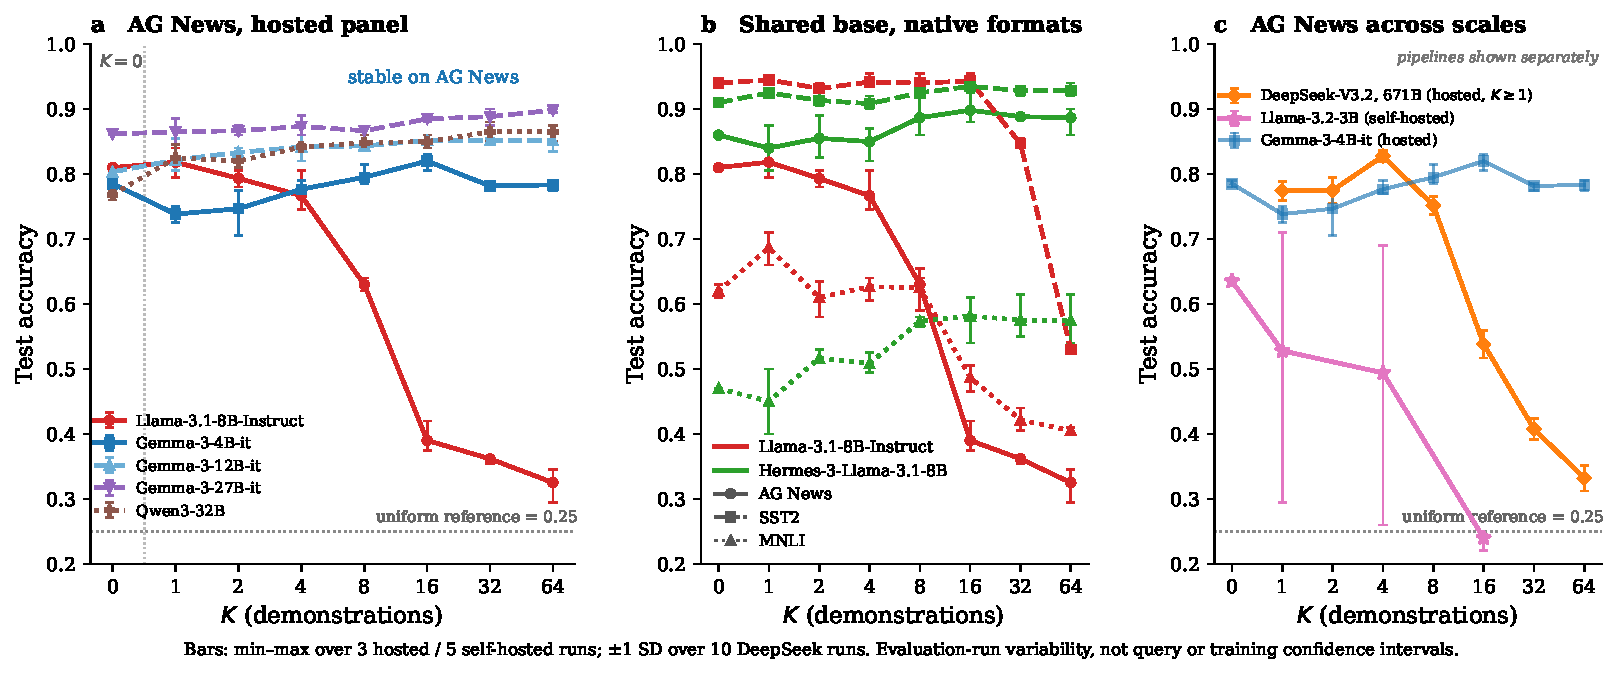
\includegraphics[width=\textwidth]{figures/revision/final_behavioral_panel.pdf}
\caption{\textbf{Many-shot accuracy curves differ across model--task pairs.} \textbf{a},~Accuracy versus the number of demonstrations $K$ on ag\_news for five models on the hosted panel, including the zero-shot baseline at $K{=}0$ (dotted separator). Llama-3.1-8B-Instruct peaks at $0.818$ at $K{=}1$, is below its $K{=}0$ baseline of $0.810$ by $K{=}2$, and collapses to $0.325$ by $K{=}64$, above the $0.25$ reciprocal-of-classes reference; the Gemma-3 family and Qwen3-32B remain stable or improve. Note that the models without the reported decline do not start higher: Gemma-3-4B ($0.785$) and Qwen3-32B ($0.768$) begin below Llama-3.1-8B. \textbf{b},~The within-base-model dissociation. Two publicly released post-training recipes over the \emph{same} Llama-3.1-8B base checkpoint, on three tasks: the Meta recipe collapses on all three while the NousResearch recipe (Hermes-3) does not, with \textcolor{blue}{nominal scale and base architecture shared, but native formatting and bundled
post-training changes differing.} \textbf{\textcolor{blue}{c}}\textcolor{blue}{,}~\textcolor{blue}{Scale alone does not determine these observed endpoints}: DeepSeek-V3.2 (671B) falls off the cliff while Gemma-3-4B (4B) does not, and Llama-3.2-3B falls at 3B. \textcolor{blue}{Bars show recorded min--max over three hosted evaluation runs (a,b and Gemma in c)
or five self-hosted runs (Llama-3.2-3B in c); DeepSeek bars show $\pm1$ reported
standard deviation over ten runs. These describe evaluation-run variability,
not query- or training-level confidence intervals. JSON cells score 200 queries;
repeated $K{=}0$ records add no independent zero-shot observations. Pipelines} are
not pooled; DeepSeek-V3.2 has no measured $K{=}0$ cell.}
\label{fig:regime}
\end{figure}

We evaluated many-shot ICL across an eight-model panel from four providers (3B--671B
parameters) on seven natural classification tasks spanning topic classification,
sentiment and natural-language inference, sweeping $K$ from zero into the many-shot
regime (Methods). Two qualitatively distinct behaviours emerge (Fig.~\ref{fig:regime}).
In \emph{cliff-prone} \textcolor{blue}{model--task pairs, accuracy falls substantially over the measured
$K$ range, without requiring a stable or improving low-$K$ interval}. On ag\_news,
Llama-3.1-8B-Instruct peaks at $0.818$ at $K{=}1$, is already below its zero-shot baseline
of $0.810$ by $K{=}2$ ($0.793$), and falls to $0.325$ by $K{=}64$: a drop of $49.3$
percentage points from peak, \textcolor{blue}{or $48.5$ points from zero-shot. The endpoint is above the
$0.25$ reciprocal-of-classes reference}. DeepSeek-V3.2 shows the same shape, peaking at
$0.828$ at $K{=}4$ and falling to $0.332$ at $K{=}64$. \textcolor{blue}{Separate self-hosted descriptive curves also show declines for DeepSeek-7B-chat and InternLM2.5-7B; this does not imply a decline under every query/prompt protocol. In particular, the verified regional panel below has a stable untreated InternLM endpoint.} The reported
Gemma-3, Qwen3-32B and Llama-3.3-70B curves improve or remain stable \textcolor{blue}{on the illustrated
tasks. Native templates differ between models. On a separate 500-query AG News panel,
Llama-3.1-8B declines from $0.830$ at $K{=}0$ to $0.382$ at $K{=}16$
(drop $44.8$ percentage points, pointwise 95\%} \textcolor{blue}{query/draw bootstrap interval
$[34.9,55.1]$); its empirical-majority reference is $0.286$ and only 24 of 18,000
outputs are invalid. Label-distribution and order controls do not establish
invariance} to demonstration order (Supplementary Notes~7--8).

\textcolor{blue}{On the 200-query controlled AG News panel, contextual calibration raises raw complete-label likelihood accuracy at $K{=}16$ from $0.307$ to $0.733$ (gain $42.6$ percentage points, pointwise 95\%} \textcolor{blue}{interval $[33.4,51.5]$); greedy generation scores $0.463$ on the same prompts. Calibrated accuracy still declines from $0.815$ at $K{=}0$ to $0.653$ at $K{=}32$. Bias correction therefore explains a substantial readout-dependent component without establishing a capacity mechanism. Separate development order and final-label controls give class-dependent responses rather than uniform copying (Supplementary Notes}~\textcolor{blue}{7--8).}

The $K{=}0$ baseline provides an accuracy reference for comparing where the curves
start. On ag\_news, models without the reported decline do not simply start higher.
Gemma-3-4B ($0.785$) and Qwen3-32B ($0.768$) begin \emph{below} Llama-3.1-8B ($0.810$),
yet hold or gain while Llama loses $48.5$ percentage points relative to zero-shot. The
ratio $a_{64}/a_{0}$ summarizes the high-$K$ endpoint relative to that baseline: on
ag\_news it is $0.40$ for Llama-3.1-8B against $1.00$ (Gemma-3-4B), $1.06$
(Gemma-3-12B), $1.04$ (Gemma-3-27B) and $1.13$ (Qwen3-32B). \textcolor{blue}{These examples show that
the different endpoints are not explained by a higher starting accuracy alone.}

Regime membership is reported per model--task pair, because the same model can be
cliff-prone on one task and stable on another: Llama-3.1-8B collapses on ag\_news, sst2
($0.940\rightarrow0.530$) and MNLI ($0.620\rightarrow0.405$), whereas its reported dbpedia
and imdb \textcolor{blue}{curves do not show the same decline. The examples span scales:} a 3B and a 671B
model show declines, while selected 4B and 70B curves do not (Supplementary Table~4).
\textcolor{blue}{They do not establish a panel-wide absence of association with scale or architecture.
The within-base-model comparison contrasts Llama-3.1-8B-Instruct, with}
$a_{64}/a_{0}{=}0.40$ on ag\_news\textcolor{blue}{, and Hermes-3-Llama-3.1-8B, with $a_{64}/a_{0}{=}1.03$
(Fig.}~\textcolor{blue}{\ref{fig:regime}}\textcolor{blue}{b). Nominal scale and base architecture are shared, but native
templates and bundled training ingredients differ. This pair therefore associates
released recipes with different curves rather than isolating a responsible alignment
component or an axis independent} of long-context training~\cite{zou2025manyiclbench}\textcolor{blue}{.
On MNLI, Llama-3.1-8B changes from $0.620$ to $0.405$ and Hermes from $0.470$ to $0.575$ between $K{=}0$ and $64$ (Supplementary Fig.}~\textcolor{blue}{4); their endpoint ratios use different zero-shot denominators.}

\textcolor{blue}{On the same controlled panel, native-format accuracy at $K{=}0/16/32$ is $0.850/0.463/0.318$ for Instruct and $0.880/0.898/0.916$ for Hermes. Under identical neutral-format prompts, both descendants produce only invalid labels; the base checkpoint is $74.5\%$ invalid at $K{=}0$ and $100\%$ invalid at $K{=}16,32$. This output-format sensitivity prevents attributing the native-curve difference to alignment or locating its origin in post-training (Supplementary Note}~\textcolor{blue}{8).}

\textcolor{blue}{A separate shared-prompt panel resolves a distinction that strict generation alone cannot. At $K{=}32$, complete-label likelihood accuracy is $88.17\%$ for Base, $88.67\%$ for Instruct and $88.83\%$ for Hermes, despite no valid strict generated labels from either descendant. Thus the native-format contrast does not generalize to this restricted-label readout. In the released T\"ulu 3 series, strict accuracy at $K{=}32$ is $34.67\%$ after SFT, $85.83\%$ after DPO and $88.50\%$ in the final checkpoint; corresponding validity is $39.67\%$, $96.17\%$ and $99.83\%$. Label-likelihood accuracy remains $87.33$--$88.67\%$. The DPO-minus-SFT difference in the $K{=}32$ versus $4$ trajectory is $50.50$ points $[29.50,71.00]$ for generation but $0.67$ points $[-2.00,2.83]$ for likelihood. This is a stage-associated compliance difference, not an isolated causal effect of a training ingredient (Supplementary Note~9).}

\textcolor{blue}{A bounded $2\times2$ count/length study crosses $K{=}4,16$ with two matched prompt-token budgets. All 2,400 outputs are valid and no cliff appears under these compact stimuli. Both fixed-count length-effect likelihood intervals include zero. The matched-budget count effect is $+6.33$ points $[-3.17,18.33]$ at the lower budget and $+9.83$ points $[1.83,19.50]$ at the higher budget. Source-linked shortening changes content as well as compression; these results do not show that count causes the original decline or rule out length effects at other budgets.}

\subsection{The logit lens and region-restricted fine-tuning}\label{subsec:locus}

\begin{figure}[t]
\centering
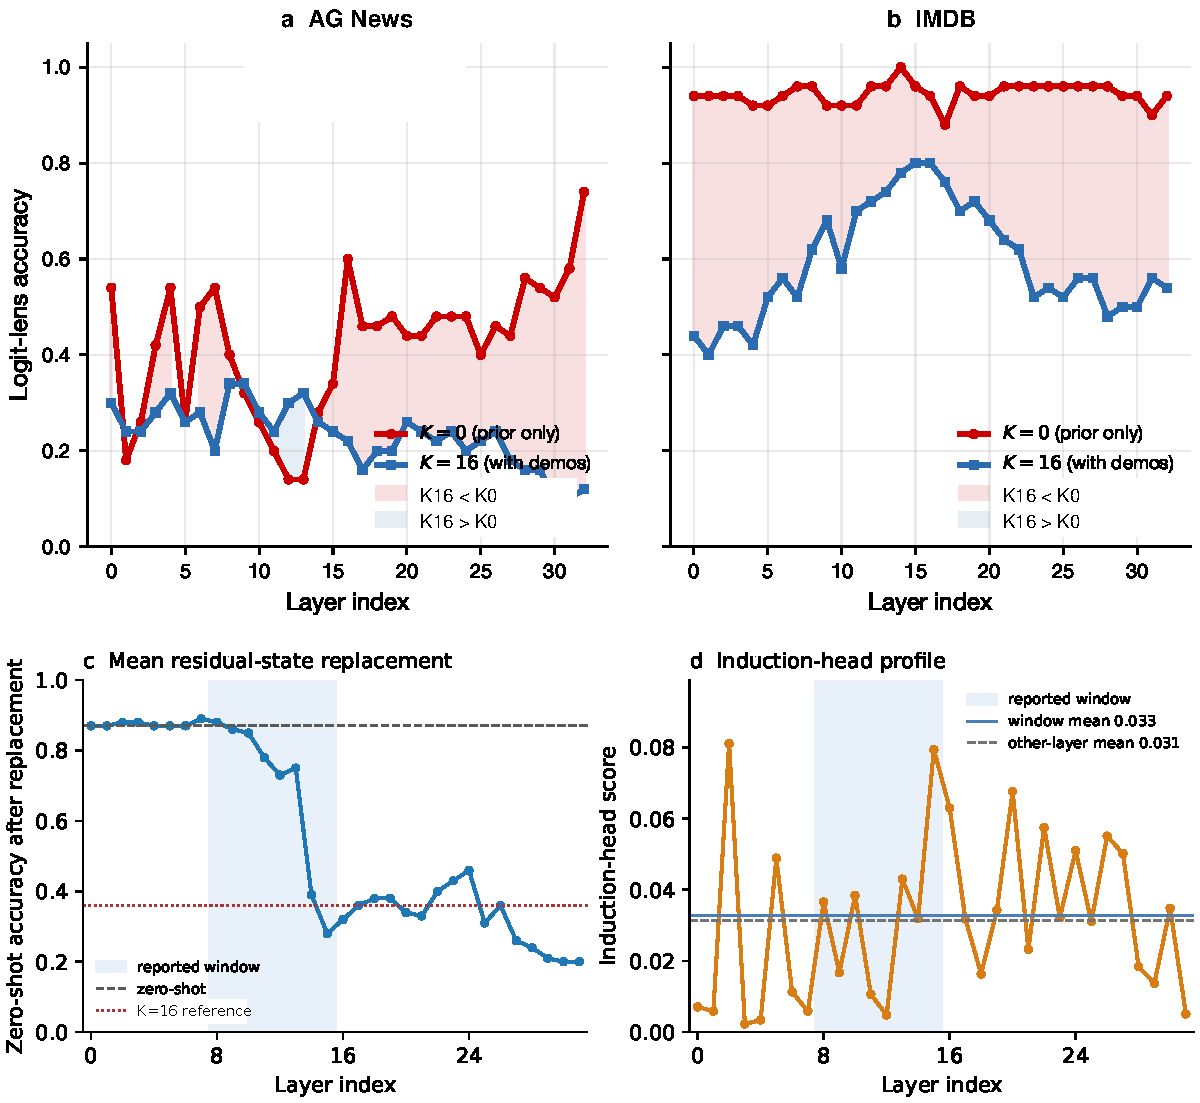
\includegraphics[width=\textwidth]{figures/revision/final_mechanistic_readouts.pdf}
\caption{\textbf{\textcolor{blue}{Layer-resolved readouts and state interventions.}} \textbf{\textcolor{blue}{a,b}}\textcolor{blue}{,}~\textcolor{blue}{Raw logit-lens label readout at $K{=}0$ and $K{=}16$ for AG News and IMDB. The enlarged curves show descriptive output-head readouts; no query-level uncertainty is assigned to these panels.} \textbf{\textcolor{blue}{c}}\textcolor{blue}{,}~Llama-3.1-8B, ag\_news, $K{=}16$\textcolor{blue}{: zero-shot accuracy after replacing a layer's query-position residual state with its mean in-context task state}. The profile tracks the zero-shot baseline ($0.87$) through layer~10, declines from layer~11 ($0.78$) and drops sharply at layer~14 ($0.39$), close to the collapsed in-context accuracy of $0.36$. Values stay low to the end of the stack, marking a transition rather than a bounded band. \textbf{d},~Induction-head score per layer. The two largest values are at layers~2 ($0.081$) and~15 ($0.079$), but only the second lies inside the comparison band, blocks 8--15; layer~20 is nearly as high\textcolor{blue}{. The means inside ($0.033$) and outside ($0.031$) are descriptive, without an equivalence analysis. We report this profile} as a negative result rather than as convergent \textcolor{blue}{localization evidence. Panels c,d show the per-layer state-replacement and induction-score profiles.}}
\label{fig:mech}
\end{figure}

Where in the network does the cliff arise? A logit-lens
analysis~\cite{nostalgebraist2020logit}, which projects intermediate activations through
the output embedding, traces where the correct label becomes \textcolor{blue}{readable through that
fixed head (Fig.}~\textcolor{blue}{\ref{fig:mech}}\textcolor{blue}{a,b). Readability through one head does not establish all
linear decodability or a causal failure locus}~\textcolor{blue}{\cite{belrose2023tunedlens}}\textcolor{blue}{. To examine
where a localized fine-tune can compensate,} we performed region-restricted fine-tuning:
a brief low-rank adaptation (Methods) confined to a contiguous band of transformer
blocks, scored as \emph{cliff recovery}, the change in accuracy at the \textcolor{blue}{selected
demonstration count. Successful compensation need not locate the original deficit.}

\textcolor{blue}{We evaluate exact-target regional adapters on a fresh AG News panel, retaining both zero-shot and contextual performance (Fig.~\ref{fig:causal}; Table~\ref{tab:recovery}). Across three independent calibration/training blocks per band, Llama-3.1 early and middle adapters reach $87.28\%$ and $85.22\%$ accuracy at $K{=}16$, versus $28.50\%$ untreated and $72.89\%$ after late adaptation. However, early/middle zero-shot accuracy is only $0.33\%/1.00\%$, with valid-label fractions $0.67\%/1.00\%$, versus late accuracy $83.33\%$. Thus high-$K$ improvement does not imply harmless repair. The paired early-minus-late high-$K$ difference is $14.39$ percentage points (pointwise 95\% interval $[-1.67,33.00]$); middle-minus-late is $12.33$ points $[1.50,30.56]$. These few-block intervals do not establish a universal regional ordering. Exact targeting is verified for this cohort; nominal depth/component summaries with incomplete targeting records remain descriptive supplementary evidence, not support for a localized failure.}


Two \textcolor{blue}{further layer-resolved measures characterize the comparison
(Fig.}~\textcolor{blue}{\ref{fig:mech}}\textcolor{blue}{c,d). Mean residual-state replacement} tracks the zero-shot baseline
($0.87$) through layer~10, declines from layer~11, and drops sharply at layer~14 to
$0.39$, close to the collapsed in-context accuracy of $0.36$. The onset falls inside the reported window, but the profile stays low to the end of
the stack and therefore marks a transition rather than a bounded band.
\textcolor{blue}{This full-state replacement differs from selecting and aggregating attention-head outputs
in published function-vector procedures}~\textcolor{blue}{\cite{hendel2023taskvectors,todd2024functionvectors}}\textcolor{blue}{;
its harmful zero-shot effect does not demonstrate a beneficial task vector or locate the
original many-shot deficit.} The induction-head score~\cite{olsson2022induction} has its
two largest values at layers~2 and~15, with mean $0.033$ within blocks 8--15 and $0.031$
outside. We report the induction-head profile as a negative result\textcolor{blue}{, rather than treating
the closeness of these means as equivalence or using it to establish an
integration/readout circuit.}

\subsection{Regional adaptation and controlled state transfer}\label{subsec:causal}

\begin{figure}[t]
\centering
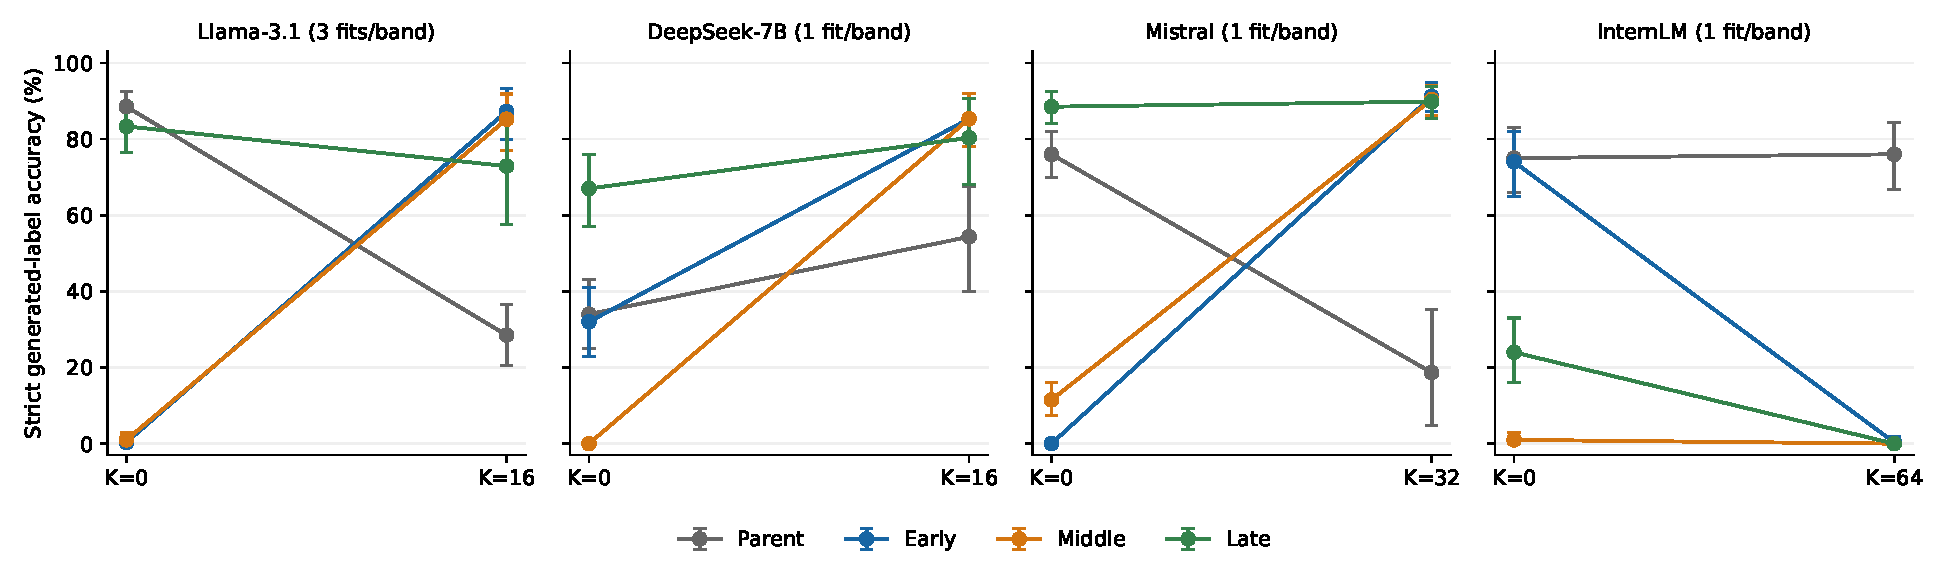
\includegraphics[width=\textwidth]{code/publication/generated/regional_tradeoffs.pdf}
\caption{\textbf{\textcolor{blue}{Regional adaptation trades contextual performance against zero-shot output compliance.}}
\textcolor{blue}{Strict generated-label accuracy on AG News, with invalid outputs counted as incorrect. Only $K{=}0$ and the indicated endpoint are measured; connecting segments are visual guides, not estimated intervening curves. Llama-3.1 averages three independent calibration/training blocks per band; the other checkpoints have one fit per band. All have three paired endpoint demonstration draws and one zero-shot measurement per query/adapter, with 200 queries for Llama-3.1/Mistral and 100 for DeepSeek/InternLM. Error bars are pointwise 95\% crossed bootstrap intervals; for one-fit cells they describe query/draw uncertainty conditional on that fit. Table~\ref{tab:recovery} and Supplementary Note~9 report validity and paired comparisons. Early/middle gains do not imply preserved zero-shot behavior, and all three InternLM adapters harm the contextual endpoint.}}
\label{fig:causal}
\end{figure}

\textcolor{blue}{Across the other checkpoints, no single region dominates both endpoints. DeepSeek-7B early/middle adapters reach $85.33\%$ at $K{=}16$ versus $80.33\%$ late, but late adaptation has the best zero-shot accuracy ($67.00\%$). Mistral's three adapted $K{=}32$ accuracies are similar ($91.17\%$, $90.33\%$, $89.83\%$); late adaptation also preserves valid zero-shot output and reaches $88.50\%$, whereas early adaptation produces no valid zero-shot labels. InternLM's untreated endpoint is already stable ($75.00\%$ at zero-shot, $76.00\%$ at $K{=}64$), and all adapters reduce endpoint accuracy to at most $0.33\%$, with at most $0.67\%$ valid output. Targeting, finite/nonzero gradients, changed adapter weights, frozen base weights and exact reload checks pass for all 18 adapters. These adverse outcomes are valid measurements of output behavior; without a likelihood readout in this regional panel, they do not establish erasure of task knowledge. Llama-3.2 is not included in this verified cohort because its weights were unavailable.}

\begin{table}[htbp]\centering\color{blue}\footnotesize
\caption{\textbf{Regional accuracy and output validity (\%).} Zero-shot and contextual endpoints on AG News: $K=16$ for Llama/DeepSeek, 32 for Mistral and 64 for InternLM. Means weight fits equally. Llama has three fits per band, others one; parents are shared untreated baselines. Invalid outputs count as incorrect. Three paired endpoint draws; zero-shot once per query/adapter. Query counts are 200 for Llama/Mistral and 100 for DeepSeek/InternLM. Whole-prompt supervision is used throughout; this is distinct from the query-label objective in Table~\ref{tab:controlled}.}
\label{tab:recovery}
\begin{tabular}{lrrrr}
\toprule
Model / band & $a(0)$ & $a(K)$ & Valid $0$ & Valid $K$ \\
\midrule
Llama-3.1 parent & 88.50 & 28.50 & 100.00 & 100.00 \\
Llama-3.1 early & 0.33 & 87.28 & 0.67 & 100.00 \\
Llama-3.1 middle & 1.00 & 85.22 & 1.00 & 100.00 \\
Llama-3.1 late & 83.33 & 72.89 & 92.83 & 99.33 \\
DeepSeek-7B parent & 34.00 & 54.33 & 36.00 & 97.33 \\
DeepSeek-7B early & 32.00 & 85.33 & 94.00 & 100.00 \\
DeepSeek-7B middle & 0.00 & 85.33 & 0.00 & 100.00 \\
DeepSeek-7B late & 67.00 & 80.33 & 81.00 & 100.00 \\
Mistral parent & 76.00 & 18.67 & 96.50 & 19.67 \\
Mistral early & 0.00 & 91.17 & 0.00 & 100.00 \\
Mistral middle & 11.50 & 90.33 & 12.00 & 100.00 \\
Mistral late & 88.50 & 89.83 & 100.00 & 100.00 \\
InternLM parent & 75.00 & 76.00 & 100.00 & 100.00 \\
InternLM early & 74.00 & 0.33 & 89.00 & 0.67 \\
InternLM middle & 1.00 & 0.00 & 1.00 & 0.00 \\
InternLM late & 24.00 & 0.00 & 27.00 & 0.00 \\
\bottomrule\end{tabular}\end{table}


\textcolor{blue}{Controlled state-transfer tests provide no convincing selective rescue. Within Llama-3.1, native-format generated accuracy declines from $83.00\%$ at $K{=}4$ to $44.17\%$ at $K{=}16$; complete-label likelihood declines from $84.50\%$ to $29.50\%$. Replacing query-text states at block outputs 7 or 15 with same-query healthy states changes high-$K$ generated accuracy by only $+1.17$ points $[-1.33,4.50]$ and $+0.50$ points $[-0.33,2.33]$ relative to self-patching. The larger contrast against an unrelated donor at block 7 reflects damage from that donor rather than rescue. A final-block query-only output patch has no downstream attention path to the later answer position; its zero effect is a structural control, not evidence that late states are irrelevant. These bounded tests leave the original failure locus unresolved.}

\textcolor{blue}{Reciprocal splicing of blocks 0--7, 8--15 or 24--31 between Instruct and Hermes also does not establish transfer of a cliff. Under the common prompt, parent and hybrid label-likelihood accuracy remains high, while all strict generated outputs at nonzero $K$ are invalid. All twelve paired high-minus-low likelihood-change intervals include zero. The absence of a parent likelihood cliff and the uninformative generated-label readout limit this intervention's causal test. On 50 held-out AG News language spans, late Instruct-to-Hermes splicing increases mean token negative log likelihood by $0.144$ nats ($[0.116,0.171]$), showing a compatibility cost on this bounded news-domain diagnostic. The complete controls and pilot dispositions are reported in Supplementary Note~9; neither reciprocal editing nor preserved general language competence is established.}

\textcolor{blue}{To distinguish contextual adaptation from ordinary task learning, we
compare four objectives in a fixed eight-block region (12--19), with three paired
calibration/training blocks (Table}~\textcolor{blue}{\ref{tab:controlled}}\textcolor{blue}{; Methods). At $K{=}16$,
contextual query-label training (B) exceeds zero-shot query-label training (C) by
$39.17$ percentage points (pointwise 95\%} \textcolor{blue}{interval $[20.63,56.30]$), with similar
zero-shot accuracy. The zero-shot-adjusted difference is $40.33$ points
$[22.33,56.70]$. B also exceeds shuffled-target training (D) by $64.80$ points
$[57.63,71.63]$; D itself harms high-$K$ performance. Thus contextual presentation
helps beyond this task-learning control, although input-token exposure is not matched.}

\textcolor{blue}{Whole-prompt training (A) improves $K{=}16$ accuracy to $0.894$ but
all 600 zero-shot outputs violate the strict label-only format. Raw label likelihood
still scores $0.882$ at $K{=}0$, distinguishing restricted topic discrimination from
generation compliance. Calibration adds $0.20$ points after A at $K{=}16$
($[-3.07,4.17]$), without a clear additional benefit. Full $K$ curves on a separate
100-query development panel show high-$K$ gains alongside small-$K$ format costs.
On 100 held-out SST2 queries, B scores $0.898$ at $K{=}16$ versus untreated $0.837$
(gain $6.11$ points, $[1.33,12.44]$), whereas A's zero-shot performance is highly
variable across blocks. These controls support context-dependent adaptation in one
checkpoint/task setting, not general preservation or causal localization
(Supplementary Note}~\textcolor{blue}{8).}

\begin{table}[t]
\centering
\caption{\textbf{\textcolor{blue}{Controlled training objectives on AG News.}}
\textcolor{blue}{Strict generated-label accuracy and invalid-output percentages, averaged equally
over three independently sampled calibration/training blocks; 200 shared held-out
queries and five demonstration draws at $K{=}16$, with $K{=}0$ evaluated once per
query and adapter. All arms use the same adapter region and optimizer-update
budget. B/C match query-label presentations but not input-token exposure;
A additionally supervises prompt tokens. Invalid outputs count as incorrect.
Supplementary Note}~\textcolor{blue}{8 reports every block and pointwise intervals.}}
\label{tab:controlled}
\footnotesize
\begin{tabular}{lrrrr}
\toprule
Training objective & $a(0)$ (\%) & $a(16)$ (\%) & Invalid $K{=}0$ (\%) & Invalid $K{=}16$ (\%) \\
\midrule
Untreated & 85.00 & 46.30 & 0.00 & 0.00 \\
A: contextual whole-prompt & 0.00 & 89.37 & 100.00 & 0.00 \\
B: contextual query-label & 89.50 & 93.13 & 0.17 & 0.00 \\
C: zero-shot query-label & 90.67 & 53.97 & 0.00 & 0.00 \\
D: shuffled query-label & 81.17 & 28.33 & 0.00 & 0.00 \\
\bottomrule
\end{tabular}
\end{table}

\section{Discussion}\label{sec:discussion}

We set out from a failure: for particular model--task pairs, adding correct
demonstrations to the context reduces accuracy rather than improving it. \textcolor{blue}{CLS offers a
framework for asking how rapid context use and slower adaptation in weights interact
when this happens. In-context learning provides rapid, prior-dependent adaptation,
and fine-tuning can make changes to behaviour} durable. The empirical content of the
comparison is that the reliability \textcolor{blue}{of context use varies with model and task, two
post-trained descendants of one base show contrasting curves, and regional
fine-tuning changes performance. These observations connect} prior-dependent
ICL~\cite{pan2023whaticllearns,wei2023largericldifferently}, many-shot
degradation~\cite{tang2025overprompting,zhang2025moreisnotbetter} and long-context
accuracy drops~\cite{zou2025manyiclbench}\textcolor{blue}{; whether they express a common interference
or capacity mechanism remains a hypothesis.}

This connects a fast-moving line of recent work. Induction-head circuits have been
linked to hippocampal episodic memory~\cite{jian2024icl}, the interplay of in-context
and in-weight learning has been modelled directly~\cite{russin2025iclinweight},
episodic retrieval has been argued to complement parametric
learning~\cite{lampinen2025latent}, and explicit fast-context/slow-parameter schemes
have been trained \textcolor{blue}{jointly}~\textcolor{blue}{\cite{tiwari2026fastslow}}\textcolor{blue}{. Xu and colleagues distinguish
contextual lookup from weight-based memory}~\textcolor{blue}{\cite{xu2026memo}}\textcolor{blue}{. Chan and colleagues
show how training-data distributions affect the emergence and coexistence of
in-context and in-weight learning}~\textcolor{blue}{\cite{chan2022distributional}}\textcolor{blue}{; Singh and colleagues
show that ICL can emerge and later recede during training, with evidence of competition
between contextual and in-weight strategies}~\textcolor{blue}{\cite{singh2023transient}}\textcolor{blue}{. Our contribution
is to bring this fast/slow perspective to the observed many-shot failures and their
response to regional adaptation, using CLS to organize questions about interference
and consolidation.}

\textcolor{blue}{The regional result concerns adaptation efficacy and output tradeoffs, not a causal map of the original deficit. The exact-target comparison shows large high-$K$ gains with severe zero-shot costs in Llama-3.1, little high-$K$ separation among Mistral regions, and adverse InternLM outcomes. In contrast, contextual query-label training in the fixed-band objective study improves high-$K$ performance relative to zero-shot task training without the whole-prompt objective's extreme zero-shot invalidity. These are different objectives and query panels, not interchangeable replications. The induction-head profile, raw lens and mean-state replacement answer different descriptive questions. Controlled within-model patching supplies no convincing rescue at the informative tested sites, and reciprocal splicing lacks an informative parent cliff under its primary readout. Stronger localization still requires interventions with an appropriate signal and transmission path, as in controlled causal tracing~\cite{meng2022causaltracing}.}


\textcolor{blue}{These results invite predictions testable in the same computational system. If the
cliff reflects inter-item interference among accumulating demonstration representations,
then interventions that reduce representational overlap should raise the threshold
without changing context-window length}~\textcolor{blue}{\cite{bertsch2025longicl,zou2025manyiclbench}}\textcolor{blue}{.
The bounded count/length manipulation supplies no cliff under compact stimuli; testing the hypothesis across the original long-context regime requires broader token budgets with class composition, order and truncation controlled. A CLS-inspired consolidation account
further motivates testing whether interleaved replay preserves previously learned
performance better than equally exposed fine-tuning without replay. These are
prospective tests: evidence for complementarity requires benefits beyond those of
additional supervised training alone.}

Several limitations bound these claims. Regime membership is a per-task property, not
a uniform model-level one. The recipe dissociation rests on one base checkpoint and
two recipes\textcolor{blue}{, with differing native formats; it does not identify which training or
formatting changes produce the difference}. We attempted to separate in-context
\emph{learning} from \emph{retrieval} using synthetic rules, but
the probe was uninformative and we draw no learning-versus-retrieval conclusion from
it (Supplementary Note~3). The \textcolor{blue}{regional comparisons cover classification and a limited
set of adapter budgets. Three independent training blocks cover each Llama-3.1 region; the other regional checkpoints have one fit per band. Evaluation-draw variation is not independent training
replication, and invalid outputs require separate accounting. Contextual calibration
mitigates the untreated decline; high-$K$ gains and low-$K$ format costs depend on
the training objective. Neither the self-target nor reciprocal-splicing comparisons establish reliable induction of a new cliff. The hosted DeepSeek-V3.2 zero-shot cell remains unmeasured; it cannot be supplied by the separate local DeepSeek-7B experiment.}

The account is nonetheless constructive as a research programme. One motivation for
continual learning is currency, because the world changes after the training cutoff.
\textcolor{blue}{The reported cliffs motivate a second question: can learning in weights stabilize
context use when additional demonstrations reduce accuracy? A design to test pairs} the
fast path \textcolor{blue}{of in-context learning with slower, replay-augmented fine-tuning, and
evaluates both high-$K$ gains and preservation of zero-shot and transfer performance
under matched exposure and compute. Deployment would also require a separately
validated trigger for unreliable context use}. More immediately, the regional results
justify testing whether adapting a small part of the network can improve many-shot
performance reliably under these controls.

\section{Methods}\label{sec:methods}

\subsection{Models and access}
The cross-model panel comprises eight instruction-tuned models from four providers
(3B--671B parameters), selected to span scales and model families:
Llama-3.1-8B-Instruct, Llama-3.2-3B-Instruct and Llama-3.3-70B-Instruct (Meta); Gemma-3
at 4B, 12B and 27B (Google); Qwen3-32B (Alibaba); and DeepSeek-V3.2 (DeepSeek).
Behavioural sweeps \textcolor{blue}{combine hosted and self-hosted pipelines, identified separately.
Hosted comparisons do not control provider-specific decoding, reasoning or
system-prompt} settings. The zero-shot ($K{=}0$) anchor is available for the six models
run on the hosted panel that includes $K{=}0$; ratios of the form $a_{64}/a_{0}$ are
reported only for those models, and every such ratio is computed within a single
pipeline. Because hosted and self-hosted runs give slightly different zero-shot values
for the same model and task (for Llama-3.1-8B on ag\_news, $0.81$ hosted, $0.85$
self-hosted at $n{=}200$, $0.87$ in the mechanism run at $n{=}100$), we never subtract
across pipelines, and every before/after comparison is within-run. The logit-lens,
regional fine-tuning and mechanism analyses require access to hidden states and weights
and were run on self-hosted open-weight checkpoints\textcolor{blue}{. Native chat templates differ
between models;
architecture, tokenizer and provider are not independently manipulated. The controlled self-hosted experiments use BF16 without quantization; the
cross-model panel does not identify an effect of quantization.}

\subsection{Classification tasks}
The seven-task panel spans topic classification (ag\_news, dbpedia), sentiment
(sst2, imdb, electronics reviews), natural-language inference (MNLI) \textcolor{blue}{and emotion
classification (tweet\_}\textcolor{blue}{emotion). QNLI and TREC are additional evaluations with
coverage specified in the supplement}. For each task we use the standard label set.
Demonstrations are \textcolor{blue}{sampled using per-class quotas; the panel sampler uses
$\max(1,\lfloor K/C\rfloor)$ examples per class and then slices to $K$. With sufficient
class supplies this gives} 60 rather than 64 demonstrations for \textcolor{blue}{six-class TREC at
requested $K{=}64$, while still returning $K$ when $K<C$. Recorded query counts vary:
the selected Llama-3.1, Llama-3.2 and Mistral regional runs use 200 queries per draw,
whereas selected DeepSeek-7B and InternLM2.5 runs use 100
(Supplementary Table}~\textcolor{blue}{S11}). Query sets are \textcolor{blue}{not necessarily class-balanced.
The controlled AG News panel uses disjoint query, calibration and demonstration
pools and has an empirical-majority reference of $0.275$; the separate 500-query
panel has a reference of $0.286$. Majority rates are not inferred from aggregate
accuracies for panels without query-label records.}

\subsection{Many-shot prompt construction and decoding}
For a given task and $K$, the prompt concatenates a fixed natural-language
instruction, $K$ demonstrations sampled without replacement from the demonstration
pool, and a single query, formatted with the model's chat template. Within a cell, all
queries share one demonstration draw; the reported seed-to-seed spread is therefore
variability across demonstration draws. We sweep $K$ over a geometric schedule from
$0$ into the many-shot regime. Outputs are mapped to the label set by constrained
string matching; an output matching no label is recorded as \emph{unparseable} and
scored as incorrect\textcolor{blue}{. Total accuracy therefore includes invalid outputs as errors;
accuracy conditional on valid labels must retain its valid/invalid denominator. The supplementary behavioural-validity table gives per-cell counts and their coverage}.
In self-hosted intervention runs, some long-context cells degenerate to no parseable
output at all; these are identified as decode failures \textcolor{blue}{(Table}~\textcolor{blue}{\ref{tab:recovery}}\textcolor{blue}{).
Parseable mistakes do not by themselves identify an integration failure. Controlled experiments record exact prompt lengths and reject overflow; none of
their prompts is truncated or rejected. The dedicated count/length factorial uses compact source-linked stimuli and matched token budgets (Supplementary Note~9); it does not identify a general demonstration-count capacity limit.}

\subsection{Defining and detecting the cliff, and regime classification}
For each measured model--task pair we obtain an accuracy-versus-$K$ curve. The peak
accuracy $a_{\max}$ is the maximum over available $K$, including $K{=}0$ where measured.
Because a model can be cliff-prone on some tasks and stable on others, regime is reported
per model--task pair\textcolor{blue}{. We use the term descriptively for substantial within-pipeline declines rather than
as a threshold-based population classification, and report absolute curves and
selected evaluation $K$ values. The controlled Llama-3.1/AG News study fixes
$K{=}16$ using a separate 100-query development panel: the first measured $K$
with at least $0.10$ absolute and $0.20$ peak-relative decline. This development
rule does not define the other panel tags and does not select a
threshold from the 200-query test outcomes.}

\subsection{Within-base-model recipe dissociation}
The dissociation compares two publicly released post-training recipes over the same
named base model: Llama-3.1-8B-Instruct (Meta) versus
Hermes-3-Llama-3.1-8B (NousResearch\textcolor{blue}{). Nominal scale and base architecture are shared,
but native templates and bundled SFT, preference, long-context and other training
choices are not held fixed. The comparison therefore associates this pair of released
recipes with different curves rather than attributing the difference to one alignment
ingredient, provider or training stage.}

\subsection{Logit-lens analysis}
We project the residual-stream activation at the final query position, at each layer,
through the model's output embedding~\cite{nostalgebraist2020logit}, restricting the
vocabulary to the task label tokens, and record at each layer whether the correct label
is the argmax. This measures where the prediction becomes \emph{readable} at the
output head, \textcolor{blue}{rather than where all task information is linearly decodable or where the
failure is caused. A tuned affine lens addresses a different readout assumption; the reported
raw-lens profiles do not estimate that alternative}~\textcolor{blue}{\cite{belrose2023tunedlens}}\textcolor{blue}{.}

\subsection{Region-restricted fine-tuning}
\textcolor{blue}{The verified regional cohort uses attention-projection LoRA of contiguous eight-block bands with all base weights frozen. Llama-3.1, Mistral and InternLM use blocks 0--7, 12--19 and 24--31; the 30-block DeepSeek uses 0--7, 11--18 and 22--29. Exact module names and parameter counts are in Supplementary Note~9 and the supplied execution manifest. All use rank 16, alpha 32, dropout 0.05, learning rate $2\times10^{-4}$, two epochs and gradient accumulation four, with whole-prompt next-token supervision. Llama-3.1 has three independent calibration/training blocks per region, the others one. This objective is distinct from the contextual query-label objective B below. Nominal depth, component and reverse-direction records without authenticated original targets are retained only as descriptive supplementary observations.}


\subsection{Calibration set and recovery metric}
\textcolor{blue}{Regional calibration uses AG News: 500 examples with $K{=}8$ for Llama-3.1, 300 with $K{=}16$ for DeepSeek, 500 with $K{=}32$ for Mistral and 100 with $K{=}64$ for InternLM. Evaluation uses a shared 200-query panel for Llama-3.1/Mistral, a declared 100-query subset for DeepSeek/InternLM, three paired demonstration draws at the contextual endpoint and one zero-shot measurement per query/adapter. Only these two endpoints are evaluated for this cohort. Different calibration budgets and endpoints prevent a matched architecture-effect inference. We report accuracy and validity jointly, with $R(K)=a_{\mathrm{after}}(K)-a_{\mathrm{before}}(K)$ and $S(K)=R(K)-R(0)$. Positive specificity can arise from zero-shot damage and does not establish selective repair.}


% Protocol and validity tables are in Supplementary Tables S11--S12.


\medskip\noindent\textbf{\textcolor{blue}{Controlled fine-tuning and readouts.}}\label{subsec:controlled}
\textcolor{blue}{The controlled AG News study uses Llama-3.1-8B-Instruct, native formatting, BF16
and rank-16 attention LoRA (alpha 32) in blocks 12--19: 32 projection modules and
3,407,872 trainable parameters. Each of three paired blocks uses an independent
500-query calibration sample and training seed, two epochs, learning rate
$2\times10^{-4}$, gradient accumulation four and 250 optimizer updates. Objectives
A--D are defined in Table}~\textcolor{blue}{\ref{tab:controlled}}\textcolor{blue}{; shuffled targets preserve marginals
and retain chance-correct assignments. Evaluation shares 200 held-out queries and
five demonstration draws at $K{=}16$, with $K{=}0$ once per query/adapter; queries
exclude the 500-query behavioural panel and all development/calibration/demo pools.
Greedy generation has a ten-token cap and strict complete-output parsing.
Complete-label likelihood sums token log probabilities without length normalization;
calibration subtracts the log of the arithmetic-mean label probabilities over}
\texttt{\textcolor{blue}{N/A}}\textcolor{blue}{,} \texttt{\textcolor{blue}{[MASK]}} \textcolor{blue}{and the empty query, separately by model/adapter and
context. Supplementary Note}~\textcolor{blue}{8 specifies the full protocols, descriptive $K$ curves,
native/common formats and SST2 transfer evaluations.}

\subsection{Self-target reverse-direction diagnostic}
\textcolor{blue}{The selected reverse-direction protocol applies early-band fine-tuning to Gemma-3-4B,
which shows no ag\_}\textcolor{blue}{news} collapse in its before-intervention sweep. The supervision
target reinstates the zero-context prediction: the calibration target for each example
is the label the model itself emits with no demonstrations. When that zero-shot
generation does not parse to a label, the target falls back to the first label in the
task's label set. An audit of 500 examples found that every generation
parsed, the fallback never fired, and targets agreed with the gold label on $81.6\%$
of examples (Supplementary Note~5); the audit applies to this supervision protocol. We measure accuracy across the available $K$ sweep before
and after, comparing early- \textcolor{blue}{and late-band fine-tuning. This self-generated supervision
differs from gold-labelled training and does not by itself establish new-cliff induction.}

\subsection{Mechanistic measures}
The \emph{induction-head score}~\cite{olsson2022induction} is, for each attention head, the
attention mass placed on the token immediately following a previous occurrence of the
current token, averaged over heads and aggregated by layer. Mean residual-state
replacement averages a layer's task representation over in-context examples and patches
it into a zero-shot forward pass at the same layer\textcolor{blue}{. It differs from selecting and aggregating head outputs
in published function-vector procedures}~\textcolor{blue}{\cite{hendel2023taskvectors,todd2024functionvectors}}\textcolor{blue}{;
its effect can depend on state scale and recipient compatibility. Both measures
use $n{=}100$ queries and} are reported by layer.

\subsection{Statistics}
\textcolor{blue}{The exact-target regional cohort and other new paired tests use 5,000 crossed percentile-bootstrap resamples (seed 20261116), jointly resampling paired query IDs, demonstration draws and training/calibration blocks where available. K=0 is measured once; sharing it across paired contrasts does not create independent observations. For single-fit checkpoints intervals are conditional on that fit. Nominal supplementary comparisons retain descriptive evaluation-draw ranges.
The controlled study averages all three calibration/training blocks equally and
reports pointwise 95\%} \textcolor{blue}{crossed percentile-bootstrap intervals from 2,000 resamples
(seed 2026110499), jointly resampling paired query IDs, demonstration draws and
training blocks. Training seed and calibration sample vary jointly; their separate
variance components are not identified. Five draws and three training blocks limit
interval coverage; no familywise, noninferiority or general-preservation inference
is made. Cells with entirely invalid outputs are output-contract failures; partial-invalid
cells retain valid/invalid denominators. No training-level Welch tests are assigned
to fixed-adapter regional draw summaries.}

\subsection{Compute, implementation, and availability}
Self-hosted analyses were implemented in PyTorch with the Hugging Face Transformers and
PEFT libraries\textcolor{blue}{. Controlled experiments run locally on Apple Silicon with the MPS
backend. Pinned model/data revisions, software versions, optimizer settings,
prompt/token records and saved-adapter manifests are specified in Supplementary Note}~\textcolor{blue}{8.}

\section*{Data Availability}
The cross-model and regional result JSON files are available at
\url{https://github.com/anomsubmission/LLM_Context_Collapse}\textcolor{blue}{. Controlled-study
summary data, validity counts, label distributions, confusion matrices and paired
contrasts accompany the supplementary analysis. The publication package includes the final follow-up generated text, label scores, query identities and calibrated priors used for CPU reanalysis. Full prompt/token metadata and saved adapters are available from the authors on request. The
supplementary inventory identifies the source and coverage of every regional
result; duplicate byte-identical files are counted once}. No proprietary or
personally identifying data were used.

\section*{Code Availability}
Code for prompt construction, ICL evaluation, logit-lens analysis, region-restricted
LoRA fine-tuning, mechanistic measures, calibration and figure generation is
available under the MIT licence at
\url{https://github.com/anomsubmission/LLM_Context_Collapse}. \textcolor{blue}{Source snapshots and
configuration manifests specify the controlled experiments and analyses. The accompanying publication package regenerates numerical tables and figures from measured records and source summaries; raw-lens and ancillary vector artwork with unavailable query-level sources are preserved explicitly; its manifest distinguishes unavailable measurements and conditional fixed-fit inference.}

\section*{Generative AI use}
Generative AI was used during the preparation of this manuscript to assist with
drafting, language refinement and organization of the text\textcolor{blue}{, and to assist with code and analyses. The authors are responsible for the content and verification of the analyses.}

% \section*{Author Contributions}
% M.R. conceived the study, designed and implemented the experiments, performed the analyses,
% prepared the figures, and wrote the manuscript.

\section*{Competing Interests}
The authors declare no competing interests.

\bibliography{sn-bibliography}

\end{document}
